\section{Ground state DFT: Total energies and relaxation}
\label{Sec:example-Etot}

As a first and basic example, we discuss how to set up a simple
DFT total-energy calculation for a given structure in
FHI-aims. We here expand on the example provided as a testrun: The
relaxation of a H$_2$O molecule towards its
minimum-energy structure. The relevant input files
\texttt{geometry.in} and \texttt{control.in} are included in the
directory \emph{testcases/H2O-relaxation} (see Chapter
\ref{Ch:quickstart}).  

The starting geometry here is badly distorted H$_2$O, with an initial bond
angle of 90$^\circ$. For any relaxation runs, we strongly recommend a two-step
procedure: First, pre-relax the structure with \emph{light} settings down to
(say) $10^{-2}$~eV/{\AA} or so, and only then follow up with a post-relaxation
run using \emph{tight} settings or anything else. \emph{light} calculations
may easily be cheaper by a factor of 5-10 than \emph{tight} ones, and going
down a relaxation trajectory of any length can then be a trememdous waste of
computational resources. 

The test case below only includes the quick but safe prerelaxation step, 
leading to an improved geometry that is
the optimum using \emph{light} settings. Based on this resulting geometry, the
postrelaxation step with \emph{tight} settings should be simple follow-up
exercise.

\subsection*{Input files}

Turning first to \texttt{geometry.in}, we see that the basic geometry
input for FHI-aims is very simple in most cases: \keyword{atom} lines
that contain nuclear coordinates in {\AA}, together with the appropriate
\keyword{species} designation (in this case, H and O). For a spin-polarized
calculation, one might additionally want to specify initial spin moments for
selected atoms using the \keyword{initial\_moment} keyword, in order to define
a good initial spin density guess for the s.c.f. procedure.

The input file \texttt{control.in} contains all necessary
computational information regarding the desired run. Most importantly,
the \keyword{xc} keyword is required to specify the
exchange-correlation functional; FHI-aims will not proceed
without this information. The further ``physical'' specifications -- \keyword{spin},
\keyword{relativistic}, and \keyword{charge} -- are all at their
default settings (no spin-polarization, no relativity, and no charge),
but are listed explicitly to make them visible at a quick glance. This
is especially important for the \keyword{relativistic} keyword, where
the \texttt{none} setting would not be justified
for heavier elements (see Sec. \ref{Sec:rel-example}).

The next setting, \keyword{relax\_geometry}, specifies a
geometry relaxation using the \texttt{bfgs} algorithm, together with a
standard convergence criterion for the forces in the final geometry:
No force component for any atom of the relaxed structure should exceed
10$^{-2}$ eV/{\AA}. This criterion may well be set tighter
for sensitive cases, such as a starting geometry to obtain
vibrational frequencies, but not orders of magnitude tighter (for example,
do not simply use a setting of 10$^{-4}$ eV/{\AA} because it feels more
accurate -- it will only end up probing some irrelevant
numerical traits of the energy surface, for example from the finite
integration grids, with no noticeable geometry or total energy changes
resulting at all). 

The version of the BFGS optimization algorithm used here is a trust-radius
enhanced version (as compared to a straight, textbook-like BFGS implementation
which could alternatively be used, see the description of the
\keyword{relax\_geometry} keyword). By default, the convergence of the
relaxation is additionally sped up by an intelligent guess for the Hessian
matrix used in the initial BFGS step. This is done by way of a slightly
modified version of the general purpose model matrix proposed by Lindh and
coworkers \cite{Lin95}, see keyword \keyword{init\_hess}.

The \texttt{control.in} could also include other general keywords
concern the technicalities of obtaining self-consistency, which are
not mandatory and are therefore not included in this simple test case.
Examples include a broadening of occupation numbers around
the Fermi level using the  
\keyword{occupation\_type} keyword (this has no physical impact in a
molecule with a HOMO-LUMO gap but may be important in metals), a
mixing parameter \keyword{charge\_mix\_param} for the \keyword{mixer}
(nonlinear optimization of the s.c.f. cycle), and convergence criteria for 
the s.c.f. cycle. FHI-aims attempts to choose reasonable settings for
these aspects automatically in order to help avoid lengthy
mistakes. The s.c.f. criterion for density convergence,
\keyword{sc\_accuracy\_rho} in particular is set tightly by default,
in order to have forces that are already mostly converged when the
(more expensive) force computation is first done.  

In \texttt{control.in}, it remains to set the \keyword{species}
information for H and O, the elements included in
\texttt{control.in}. Normally, these settings should be obtained by
copy-pasting the relevant information from the
\emph{species\_defaults} directory, for example the 
choices in the \emph{light} or \emph{tight} subdirectory located there. Once 
this is done, the \keyword{species} defaults may still be adapted
for the purpose in question. 

\subsection*{Output stream}

We next analyze some significant parts of the standard output
produced by FHI-aims, also provided in the file
\emph{H2O.reference.out}. We emphasize that this output is kept as
human-readable as possible; it pays to actually \emph{look} into the
output, especially when something does not appear to have gone
correct. Often, a simple warning in in the initial input section or
elsewhere in the file may already tell you what is going on. Warnings can also
be identified by ``grepping'' for asterisks in the file.

The standard output stream is structured as follows:
\begin{itemize}
  \item A summary of the setup (nodes used, required fixed dimensions,
    information in \texttt{control.in} and \texttt{geometry.in}) and,
    importantly, default values inserted for parameters that were
    \emph{not} explicitly specified in \texttt{control.in}.
  \item Preparation of fixed parts of the calculation -- most
    importantly, information regarding the setup of the per-species
    basis 
  \item Initialization -- information on the setup of all
    three-dimensional integrations, and solution of the first
    Kohn-Sham eigenvalue problem for the initial
    superposition-of-free-atoms electron density.
  \item Process and total energy information for each successive
    s.c.f. iteration.
  \item Upon convergence of the s.c.f. cycle, the Kohn-Sham
    eigenvalues are also included, as well as final total energies and
    forces in a long format for reading by external utilities (scripts
    etc.) 
  \item This is followed by information on the geometry optimization,
    up to the coordinates predicted for the next step, based on the
    converged forces obtained from the previous iteration. 
  \item Reinitialization, s.c.f., and geometry optimization
    information is repeated for each successive geometry step until
    the optimum geometry is found within the force tolerance specified
    by \keyword{relax\_geometry}.
\end{itemize}

Key information that should be paid attention to is the following:

\emph{Eigenvalue and total energy information:} \\
This should be checked for roughly realistic total energy values, a
reasonable eigenvalue spectrum: Make sure that the expected core
states, the correct number of eigenstates, and possibly the expected
HOMO-LUMO gap are all in place.

As in all other iterations, \emph{three} variants of the total energy
are given (here quoted from the \emph{initialization} step, just prior to the
start of the s.c.f. cycle for the initial geometry):
{\small
\begin{verbatim}
  | Total energy                  :         -76.44577740 Ha       -2080.19544233 eV
  | Total energy, T -> 0          :         -76.44577740 Ha       -2080.19544233 eV
  | Electronic free energy        :         -76.44577740 Ha       -2080.19544233 eV
\end{verbatim}
}
For systems with a HOMO-LUMO gap, these values should all be the same,
but for systems with fractional occupation numbers (metallic systems,
large \keyword{occupation\_type} setting, or degenerate levels at the
Fermi level), this is not generally the case.

For molecular systems, the meaning of fractional occupation numbers is
questionable, and we recommend to always rely on the first value, the
``Total energy''.

For metallic systems, fractional occupation numbers are
unavoidable. However, it is possible to estimate the total energy for
zero occupation broadening (``Total energy, T $->$ 0'') based on an
entropy expression associated with the fractional occupation
numbers. This estimate is based on a free electron gas argument; do not trust
it for atoms or small molecules. Bulk metals or metallic
surfaces benefit from this correction, and their total energy may be
estimated from the extrapolated total energy (``Total energy, T $->$
0'').

The ``free energy'' simply sums the total energy together
with the full entropy correction from the fractional occupation
numbers. This quantity has no physical meaning, but it is strictly
\emph{this} free energy to which our calculated forces correspond. The
reason is that fractional occupation numbers may carry an implicit
derivative of their own with respect to the nuclear coordinates. This
would enter the total energy, but this derivative is not available in
simple analytical terms in FHI-aims. 

\emph{Geometry information:} \\
After each relaxation step, the convergence of the present geometry is checked
(by monitoring the maximum remaining force component on any atom in the
structure), and the updated geometry to be treated next is printed. For
instance, the final (converged) geometry can be found near the end, in a
format that is directly suitable for a follow-up run:

{\small
\begin{verbatim}
------------------------------------------------------------
  Final atomic structure:
                         x [A]             y [A]             z [A]
            atom        -0.00000000       -0.07326324        0.00000000  O
            atom         0.76740631       -0.67036838        0.00000000  H
            atom        -0.76740631       -0.67036838       -0.00000000  H
------------------------------------------------------------
\end{verbatim}
}

By default, a version of this information is also written into a file 
\texttt{geometry.in.next\_step},
which should be used to continue a relaxation run and also to begin
a possible post-relaxation with \textit{tight} settings (this file
contains a usually much better Hessian for the structure at hand than
the starting guess).

\emph{Timing information:} \\
Finally, we note that FHI-aims also provides detailed timing
information as well as partial memory accounting for each
s.c.f. iteration, and as a summary at the end of each run. For
example, the provided test run reads similar to this: 

{\small
\begin{verbatim}
------------------------------------------------------------
          Leaving FHI-aims.
          Date     :  20171222, Time     :  232807.911

          Computational steps:
          | Number of self-consistency cycles          :           49
          | Number of SCF (re)initializations          :            5
          | Number of relaxation steps                 :            4

          Detailed time accounting                     :  max(cpu_time)    wall_clock(cpu1)
          | Total time                                 :        1.306 s           1.374 s
          | Preparation time                           :        0.083 s           0.088 s
          | Boundary condition initalization           :        0.000 s           0.000 s
          | Grid partitioning                          :        0.026 s           0.025 s
          | Preloading free-atom quantities on grid    :        0.012 s           0.012 s
          | Free-atom superposition energy             :        0.012 s           0.013 s
          | Total time for integrations                :        0.368 s           0.385 s
          | Total time for solution of K.-S. equations :        0.030 s           0.031 s
          | Total time for EV reorthonormalization     :        0.001 s           0.000 s
          | Total time for density & force components  :        0.294 s           0.308 s
          | Total time for mixing                      :        0.043 s           0.043 s
          | Total time for Hartree multipole update    :        0.046 s           0.051 s
          | Total time for Hartree multipole sum       :        0.269 s           0.286 s
          | Total time for total energy evaluation     :        0.008 s           0.009 s

          [...]

          Have a nice day.
------------------------------------------------------------
\end{verbatim}
}

The date and time at the end are in the \texttt{ddmmyyyy} and
\texttt{hhmmss.mmm} formats of a wall-clock time, \emph{not} in
seconds; i.e., the above calculation did \emph{not} take 232807~s, but
rather \emph{ended} at 23:28:07 h, one fine December 22. 

In addition, detailed timing is provided both for as elapsed CPU time
(on individual CPUs during the run), and actual elapsed wall clock
time. In a normal production run, no significant discrepancies should
occur between wall clock and CPU times. If discrepancies arise, they
could indicate serious problems with load balancing or communication
in a parallel run.  

\subsection*{Further analysis}

\begin{figure}
  \centering
  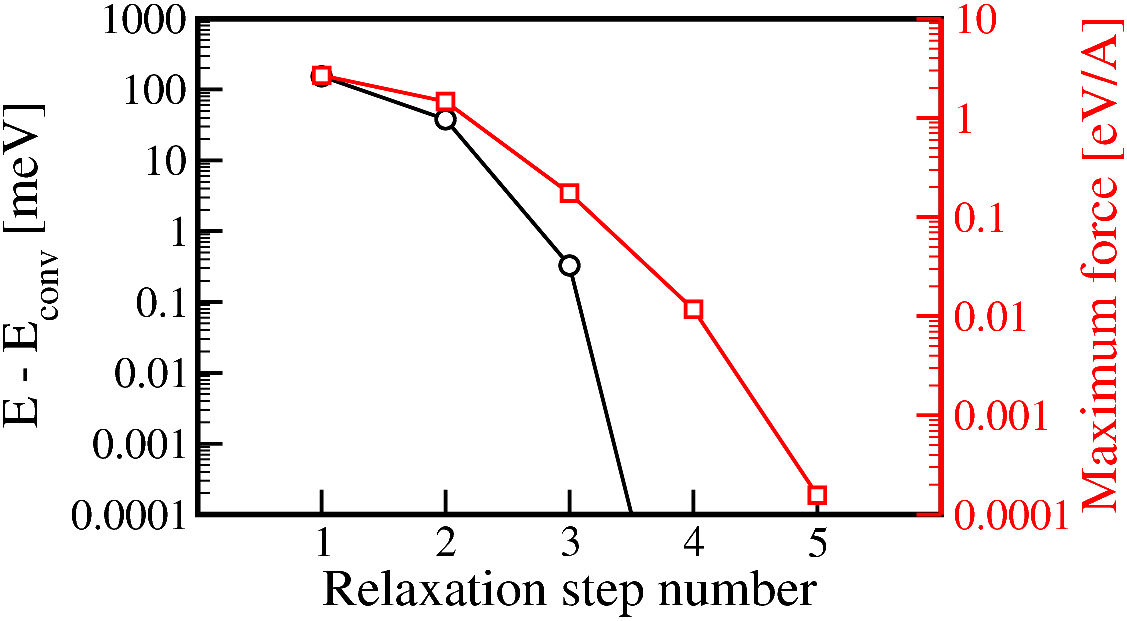
\includegraphics[width=0.7\textwidth]{H2O_trm_lindh_relaxation}
  \caption{\label{Fig:H2O-relaxation}
           Total energy convergence (left $y$ axis) and force convergence
           (right $y$ axis) during the relaxation test run of H$_2$O. A total
           of five steps is taken (initial geometry plus four relaxation
           steps). The total energy of the final step is taken as the
           reference here, and the total energy in the second-to-last step is
           already identical within the numerical accuracy of the
           calculation. The final step is only taken to bring the residual
           forces (total energy gradients) to practically zero as well.
  }
\end{figure}
Some statistics on the complete relaxation run can be obtained
using the script \\ \emph{get\_relaxation\_info.pl}, located in the
\emph{utilities} subdirectory of the FHI-aims distribution. This
script is invoked as follows:

\begin{verbatim}
  > get_relaxation_info.pl < H2O.reference.out > statistics.dat
\end{verbatim}

or with any other output file. The script searches the FHI-aims output
file for total energies (no entropy correction) and maximum force
components at the end of each relaxation step. The development of the
total energy, total energy difference with respect to the starting
geometry, and maximum force component can then be visualized as a
function of the relaxation step number, using standard tools such as
xmgrace. Fig. \ref{Fig:H2O-relaxation} visualizes the progress of the
relaxation run based on the data obtained from
\emph{get\_relaxation\_info.pl}. 

Likewise, much other information can and should be extracted from the standard
output using similar scripts. For example, the development of the geometry can
be visualized in the format of a \texttt{.xyz} file using the
\emph{create\_xyz\_movie.pl} script, using standard visualization tools such
as \texttt{jmol} or \texttt{vmd}.

To continue a relaxation run (for instance, for a post-relaxation step
with tight settings, see below), use the file
\texttt{geometry.in.next\_step} that is created by default during a
relaxation. It contains the atomic structure of the current relaxation
step, as well as the current estimate of the Hessian matrix as created
by the \option{bfgs} relaxation algorithm. This output can be
fine-tuned (or prevented) using the \keyword{write\_restart\_geometry}
and \keyword{hessian\_to\_restart\_geometry} keywords.

Obviously, all intermediate geometries (but not the Hessian) are also
part of the standard output stream by default, in the right format for
a restart.

\subsection*{Next steps}

As with any electronic structure code, \textbf{monitoring the convergence of
the basis set for each element is an important user task}, to make sure any
physical conclusions are accurate. For instance, the present example could be
continued as follows:
\begin{itemize}
  \item A ``prerelaxation'' such as the present test run should
    not employ a huge basis set, simply for efficiency's sake. The
    \emph{light} settings used for the present elements use a \emph{tier} 1
    basis set. Very often, geometries obtained with \emph{light} are already
    rather close to converged.
  \item For these same elements, you will find that the \emph{tight} settings
    actually employ \emph{tier} 2, which is significantly larger and very
    close to basis set convergence at least for DFT methods. 
  \item Obviously, one might extend this to \emph{tier} 3 or higher for test
    purposes, possibly even based on \emph{really\_tight} settings
    otherwise. Comparing the changes made between \emph{light}, \emph{tight},
    and \emph{really\_tight} settings, and different basis sets, is an 
    interesting exercise. For the H$_2$O molecule shown here, it should
    hopefully reveal that there is not much to be gained beyond what is
    prescribed as ``\emph{tight}''.
\end{itemize}
Finally, we note that ``\emph{tier} 1'' does not necessarily mean the same
level of convergence accuracy for all elements. For light elements,
\emph{tier} 2 may often be needed, and we set them by default in our
\emph{tight} settings. For significantly heavier elements (transition 
metals in particular), \emph{tier} 1  is already well converged for 
ground-state DFT calculations, which is therefore mostly the default in our
\emph{tight} settings. 
